% !TEX root = tsam_Covid19_Mexico.tex

\subsection*{Estimaciones y modelaje estocástico de dinámica de propagación en una población para distintos grupos de riesgo}

\paragraph{Participantes.} Carlos Ignacio Herrera-Nolasco, Eugenia O'Reilly-Regueiro, Sergio Iván López Ortega, Marco Arieli Herrera-Valdez. Este trabajo es parte de un reporte técnico que está siendo editado para su revisión por pares. Se pueden encontrar más detalles y referencias en \url{https://scab-unam.github.io/tsamCOVID-19/}.  

\bigskip
Sabemos que factores como la fatalidad entre casos confirmados puede depender de una diversidad de factores como la calidad de los servicios de salud, y el acceso a dichos servicios, entre otros. 
Sin embargo, es posible observar algunas similitudes macroscópicas en el comportamiento de las defunciones por COVID-19 en lugares que podría pensarse que los fallecimientos presentarían comportamientos muy distintos , como China y Korea del Sur por un lado, e Italia, por otro. 
En Korea del Sur y China, el control es muy estricto y la cuantificación de casos ha sido masiva. 
En cambio en Italia, donde la estructura poblacional es distinta, ha habido más fallecimientos por COVID19, y ha sido rebasado el sistema de salud al grado de tener que negar el uso de respiradores a la gente. 
Sin embargo, en los tres paises el cociente de fatalidad de casos (CFR por sus siglas en inglés) tiene muchas similitudes (\figref{cfrPDEdadChinaKSItalia}, panel izquierdo), que se pueden explotar para obtener las contribuciones relativas de los fallecimientos por COVID-19 (\figref{cfrPDEdadChinaKSItalia}, panel derecho) por cada grupo de edad al total de muertes observadas, y usar esas estimaciones. 

\begin{figure}[h]
\caption{CFR para distintos grupos de edad usando datos sobre fatalidad de COVID-19 de China, Korea del Sur, e Italia. El panel izquierdo muestra los CFRs de los tres países. El panel derecho, muestra las contribuciones a las muertes inferidas a partir de los CFRs. } \label{cfrPDEdadChinaKSItalia}
\begin{center}
    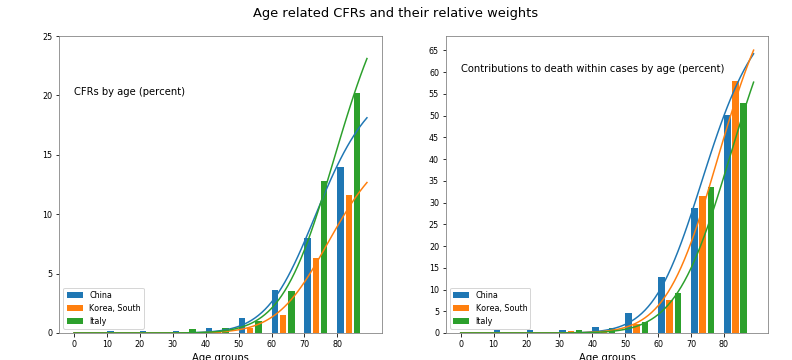
\includegraphics[width=\textwidth]{../tsam_Covid19_figures/tsam_Covid19_JHU_cfr+propDeathCases_ByAge_China+SKorea+Italy_OneFigure}
    \end{center}
\end{figure}

Por su similitud, es posible usar los pesos relativos de las defunciones de los distintos grupos de edad y  hacer distintas predicciones para el caso de México (\figrefestimates_sp}).
\begin{figure}[h]
\caption{Estimaciones de fatalidad para México tomando en cuenta grupos de edad, con los datos de China, Korea del Sur, e Italia, calculado hasta el 11 de abril de 2020, y usando un factor de ajuste por subreporte igual a 1. }. \label{estimates_sp}
\begin{center}
    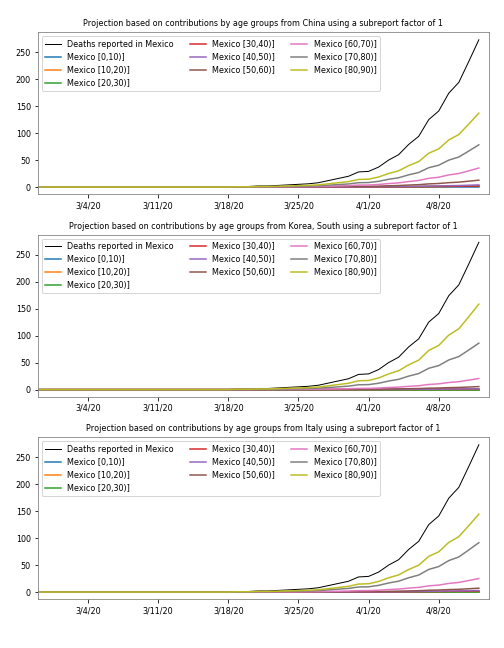
\includegraphics[width=\textwidth]{../tsam_Covid19_figures/tsam_Covid19_JHU_cfr+propDeathCasesByAgeTS_EstimatesMexico_subReportFactor1}
\end{center}
\end{figure}

Las proyecciones obtenidas usando los datos de los distintos países son similares. Hay que tomar en cuenta que estos datos no han sido ajustados con respecto a subreporte. Por ejemplo, sin ajustar los datos por subreporte, la estimación del 11 de abril de 2020 es  de alrededor 150 muertes de adultos de más de 70 años en México. 
Usando un factor de ajuste por subreporte igual a 10, estaríamos estimando que el número de muertes por COVID-19 en México sería aproximadamente 1500. 


Es importante mencionar que estas estimaciones no toman en cuenta la estructura poblacional en México, o la de los países tomados para el análisis, pero esa información está implícita en los datos de dichos países. 


\subsubsection*{Trabajo en progreso.} Estamos construyendo modelos estocásticos de dinámica de propagación basados en estimaciones cualitativas similares a las descritas arriba, con la intención de explicar mecanismos subyacentes a la propagación de la epidemia.  


